%\section{Text-based Qfact Scoring} 
%\section{Qfact Scoring by External Evidence}
\section{Qfact Confidence Scoring}
\label{sec:qfact_scoring_model}

%At the core of our column alignment method is a scoring model, giving each potential table-Qfact a likelihood score, which is used by Equation \ref{eq:likelihood}.
This section explains how we utilize external text corpora to compute 
$\textit{ext-score}(\mathcal{F})$ for the CA-score model of Section \ref{subsec:CAscore}.

The key idea is to retrieve evidence for a candidate
Qfact $(e,q,X = h_k)$, spotted from a table with Q-column $C_k$,
in a larger corpus of text, such as sentences from
Wikipedia articles.
To this end, we employ the text-based extraction
method from \cite{DBLP:conf/semweb/HoIPBW19}: a trained LSTM network 
classifies sentences that contain at least one
entity and
% at least
one quantity and tags
proper pairs of entity and quantity,
along with informative context words from the
sentence. 
Running this on Wikipedia full-text, 
% and the Stics collection \cite{DBLP:conf/sigir/HoffartMW14}, 
followed by removing duplicates and thresholding on confidence, we obtained a collection $\mathbb{C}$ of 1.6M million
Qfacts triples in the form $(e',q',X')$. By using an entity coreference resolution tool (\textit{\url{github.com/huggingface/neuralcoref}})
on two consecutive sentences and combining them
into one input, we enlarged this to a total
of 2.4M million Qfacts -- with a fair amount of
uncertainty, though. 

We treat this collection $\mathbb{C}$ as external evidence
against which we can assess Qfact
candidates distilled from web tables. 
A candidate table-Qfact $(e,q,X)$ is highly-confident if related information can be found in text, in particular, in $\mathbb{C}$.


\vspace{0.1cm}
\noindent{\bf Definition [Evidence Score].}
For Qfact $\mathcal{F} = (e,q,X = h_k)$, the evidence score from
collection $\mathbb{C}$ is:
%\hspace*{0.5cm} $\textit{ext-score}(e,C_k:q) = \max \{$\\
%\hspace*{0.5cm} $w_1 sim_1(e,e*)$ +
%$+ w_2 sim_2(q,q*) + w3 sim_3(C_k,X*)$\\
%\hspace*{0.5cm} $~|~ (e*,q*,X*) \in Ext 
%\}$\\
\begin{gather*}
\textit{ext-score}(\mathcal{F}) = \max\limits_{
(e',q',X') \in \mathbb{C} \wedge e'=e} \textit{sim}\big((q,X),  (q',X')\big)\\ 
\text{where}~~~~\textit{sim}\big((q,X),  (q',X')\big) =  w_1 \cdot \textit{sim}_1(q,q') + w_2 \cdot \textit{sim}_2(X,X')
\end{gather*}
with tunable coefficients $w_1, w_2$. The function finds the best matching evidence Qfact in $\mathbb{C}$ with same entity $e$.
% $sim_1$ gives 1 for matching entities,
%and an embedding-based relatedness score otherwise.
% and 0 otherwise.
$\textit{sim}_1$ compares quantities $q$ and $q'$
(after normalization to the same unit) and returns
a score that is 
equal
% inversely proportional 
to their
relative numeric distance $\frac{|q - q'|}{\max(|q|,|q'|)}$.
We consider a 
1\% difference as a perfect match,
because quantity values are often rounded or truncated. 
Note that if the two quantities are incomparable (from different concepts, e.g., length vs. monetary), we do not consider $(e',q',X')$ at all.
$\textit{sim}_2$ compares the Q-column header $X = h_k$ with
the evidence context bag-of-words $X'$
by the {\em directed embedding distance} of \cite{DBLP:conf/semweb/HoIPBW19}.
This rewards if the column name appears in $X'$,
but also gives credit to different words that
are related by their word2vec embeddings.
%


%%%%%%%%%%%%%%%%%%%%%%%%%%%%%%%%%%%%
\begin{comment}
\vspace{0.1cm}
We compute the likelihood of $\mathcal{F'}$ by matching it against each Qfact $\mathcal{F} = (e,q,X) \in \mathbf{C}$ collected from text documents. Here, we compute the similarity score between $\mathcal{F'}$ and $\mathcal{F}$ by matching their corresponding components. We distinguish between two types of matching, as describe below.

\vspace{0.1cm}
\noindent \textbf{Exact Entity Matching}. $\mathcal{F'}$-$\mathcal{F}$ matching belongs to this category if their entities are similar, i.e., $e' = e$. In other words, $\mathcal{F'}$ has high likelihood score if there exists similar information about the same entity $e'$ represented in text. Specifically, we give $\mathcal{F'}$ an exact entity matching score from its best matched Qfact $\mathcal{F}$ as follows:
\[
S_{\textit{exact}} (\mathcal{F}'|\mathbf{C}) = \max_{\mathcal{F} =(e,q,X) \in \mathbf{C} \wedge e = e'}\big(w_1.sim(X', X) + w_2.sim(q', q)\big)
\]
where $sim(X', X)$ and $sim(q', q)$ denotes the context and the quantity similarities between the two Qfacts, respectively; $w_1$ and $w_2$ are parameters controlling the contribution of these two scores. We define the context similarity $sim(X', X)$ using \textit{directed embedding distance (ded)}, which was proposed earlier \cite{DBLP:conf/semweb/HoIPBW19}: 
\[sim(X', X) = ded(X' \rightarrow X) = \bigg(\sum\limits_{u \in X'} W(u)\min\limits_{v \in X}(d(u,v))\bigg)\big/\sum\limits_{u \in X'}W(u)\]
where $d(u,v)$ is the semantic distance between two words $u$ and $v$, computed using word embeddings \cite{DBLP:conf/emnlp/PenningtonSM14}; $W(u)$ is the importance weight of $u$; in this case, we use \textit{idf}. For the quantity similarity, we define $sim(q', q)$ as an indicator function, which takes value of 1 if the two quantities are equals, 0 otherwise. Two quantities are considered equal if their values (after unit conversion) are at most 1\% different from each other. Note that if the two quantities are from different concepts, (e.g., length vs. monetary), we do not consider $\mathcal{F}$, as the two Qfacts are incomparable and totally unrelated.

\end{comment}
%%%%%%%%%%%%%%%%%%%%%%%%%%%%%%%%%%%%

\vspace{0.1cm}
%\noindent \textbf{Type-Related Entity Matching}. 
\noindent \textbf{Type-based Evidence.}
%
Many of the candidate facts from tables may not find
any text-based evidence by the above procedure.
This is natural, as we expect to obtain a large
number of facts from tables that cannot be spotted
in text corpora at all. If this were not the case,
we would not need to tap into tables and could instead
extract from text only.

%%%give intuition first
We can relax our notion of text evidence, however, and settle for the softer task of spotting some 
Qfact evidence with the same entity {\em type}
as the candidate at hand.
For example, to scrutinize the candidate
(\textit{Estadio Santiago Bernab\'{e}u, 81044, ``Capacity''}), we can consider the text evidence
(\textit{Old Trafford, 74140, ``Capacity''}) or (\textit{Camp Nou
, 99354, ``Capacity''}).
Intuitively, 
% the latter tells us, 
for an entity of the
same type {\small\tt stadium}, the cue word 
``Capacity'' is important and the respective quantities
fall into the same order of magnitude.
%{\color{blue}
In contrast, when examining candidates (\textit{Santiago Bernab\'{e}u, 81044, ``Capacity''}) and (\textit{Real Madrid, 81044, ``Capacity''}), 
%we hardly find any 
there is hardly any
text evidence that a {\small\tt person} or a  {\small\tt team} has a Capacity. 
%Putting into words, when talking about capacity, it is more likely that we talk about a stadium rather than a person or a team. 
% From this evidence, we link the columns as desired.
This reinforces the hypothesis that the table-based candidate is valid, including the chosen EL target (``Bernab\'{e}u'' refers to {\it Estadio Santiago Bernab\'{e}u}, not to the club president {\it Santiago Bernab\'{e}u}) and the CA inference (Capacity refers to Stadium, not to Team).
% that
% Capacity refers to Stadium, not to Team).
%}
\begin{comment}
For some potential table-Qfact $\mathcal{F'}$, it is possible that we cannot find information of the same entity $e'$ represented in text. However, we can still infer the likelihood of $\mathcal{F'}$ from other type-related entities, whose information in text can be found.
For example, looking at Figure \ref{fig:scoring}, we want to link column \textit{``Capacity''} to \textit{``Stadium''} instead of \textit{``Team''}. Suppose for stadium ``Bernabeu'', we cannot find its capacity in text from the collection $\mathbf{C}$, but we can find capacity of other stadiums, e.g., ``Allianz Arena'' is one of them
% , and even others which are not in the table
. In contrast, we cannot find any information about capacity for a team. Putting into words, when talking about capacity, it is more likely that we talk about a stadium rather than a team. From this evidence, we link the columns as desired.
\end{comment}


%%% now give formula
\vspace{0.1cm}
\noindent{\bf Definition [Type-based Evidence Score].}
%
%Specifically, for each type-related entity $e^*$ of $e'$, we compute for $\mathcal{F'}$ a type-related entity matching score as follows:
For candidate Qfact $\mathcal{F} = (e,q,X)$ and each entity $e^*$ sharing the same type with $e$, we compute a type-based evidence score of $\mathcal{F}$ with respect to $e^*$ as: 
% and text evidence
% $\mathcal{F}' = (e',q',X')$ with $e$ and $e'$ sharing the same type, their similarity is:\
% \vspace{-0.1cm}
%\[
%S_{\textit{related}}^{e^*} (\mathcal{F}'|\mathbf{C}) = \max_{\mathcal{F} =(e^*,q,X) \in \mathbf{C} } \bigg(\frac{\textit{agree}(e', e^*)}{\mathcal{Z}}\bigg)^\beta.\big(w_1.sim(X', X)\big)
%\]
\begin{align*}
    \textit{t-ext-score}(\mathcal{F}|e^*)= \max\limits_{(e',q',X') \in \mathbb{C} \wedge e'=e^*} \textit{rel}(e, e^*) \cdot \textit{sim}\big((q,X),  (q',X')\big)
\end{align*}
% \noindent As we can consider many such same-type pieces of evidence, we need to aggregate over them.
% We do this by using only the best match,
% yielding the following evidence score\\
% \hspace*{0.5cm} $\textit{t-ext-score}(e,q,C) =$\\ 
% \hspace*{0.5cm} $max_{(e^*,q^*,X^*) \in Ext} ~ rel(e,e^*)^\beta \cdot 
% sim(e,q,C~|~e^*,q^*,X^*)$\\
% where $\beta < 1$ is a tuning coefficient,
\noindent where $\textit{rel}(e,e^*)$ is the semantic relatedness between the two entities (\textit{ext-score} is actually a special case when $\textit{rel} = 1$). 
The $\textit{rel}$ function can be based on distance measures
in the underlying type taxonomy, or alternatively by the cosine
between word2vec (or wikipedia2vec) embeddings.
In our implementation, we chose the shortest Wu-Palmer 
taxonomy distance \cite{DBLP:conf/acl/WuP94} between the direct types
of two entities. This has
the advantage that we can incorporate entities $e^*$
incrementally in ascending order of distance.
%\GW{we apply this to entities, not types; entities have many types -- how exactly is the Wu-Palmer-like distance computed then? please clarify for us, may have to re-word the above, while still avoiding giving too many implementation details!}\\
This way, we efficiently prune the huge space of
potential evidence items.
%\GW{I pushed 1/Z into beta, as it is just another constant, to simplify the equation}\\
%\GW{I am not convinced about the taxonomy-distance; I would prefer embeddings, say from wikipedia2vec, but it is probably too late to change this. Hence, the wording staying a vague and leaving several options open.}\\
%\todo{Taxonomy distance is better to ensure entities have similar types (what we want), embedding is an option, but I think it captures too many thing more than just types, so being noisy. Another advantage why I choose taxonomy distance is we can do search partially by travelling on the taxonomy graph, for embedding we need to search through all candidate entities (millions of entities for yago), which is inefficient in terms of performance. But yeah, performance is not a problem as we do extraction offline. The key point is about the type-related precision}


\begin{comment}
\vspace{0.1cm}

Basically, our $S_{\textit{related}}$ is quite similar to $S_{\textit{exact}}$, where we set $w_2 = 0$, as a match in quantity should not affect the score when the two entities are different. Note that even though quantity match does not contribute to the score in this case, we still only consider Qfact $\mathcal{F}$ if $q$ and $q'$ are comparable.
$\big(\frac{\textit{agree}(e', e^*)}{\mathcal{Z}}\big)^\beta$ denotes the relatedness of $e'$ and $e^*$, i.e., penalty for this kind of matching, with $\mathcal{Z} = \log_{10}\big(\frac{\#\textit{total\_kb\_entities - 0.5}}{1.5}\big)$ is a scaling factor and parameter $\beta \geq 0$ controlling its effect (e.g., setting $\beta = 0$ will treat every entity $e^*$ as important as $e'$). 

Moreover, to restrict the search space, we only consider an entity $e^*$ as type-related to $e'$ if they are within a distance of $d$ jumps in the KB taxonomy graph (i.e., the subgraph containing only \textit{``subClassOf''} and \textit{``typeOf''} edges). For example, the distance between two sibling entities is 2. In our work, we tune and set an optimal value of $d = 4$. Choosing a higher value of $d$ will enlarge the search space and put more unnecessary noise into the model, as entities become more unrelated when we explore further. In contrast, choosing a lower value of $d$ will reduce the amount of considered Qfacts from text, resulting in the lack of information required for matching.
\end{comment}


\vspace{0.1cm}
%\noindent \textbf{Likelihood Consolidation}. 
\noindent \textbf{Combining Scores.}
A good fraction of the table-based Qfact candidates may have both kinds of text evidence: matching entities and
merely matching types.
Thus, it is natural to combine both scores.
We define the final evidence score of $\mathcal{F}$ as the average of matching evidence scores from top-\textit{k} best entities $e^*$ (including $e$ itself).
% In addition, instead of using only the best match
% from the type-based scoring, we relax this choice
% by incorporating the {\em top-k} highest-scoring
% same-type pieces of evidence.
We hypothesize that this yields a more robust signal
from the wealth of text-based evidence.

%{\color{blue}
Table \ref{table:example_ext_items} shows examples of top-scoring text evidence  for examining 
the Qfact candidate (\textit{Allianz Arena, 75000, ``Capacity''}).
%Qfact candidates 
%(which appeared in our initial example of Table \ref{table:ExampleTable}).
%}

%!TEX root = ../main.tex
\begin{table*}[t]
%{\color{blue}
	\caption{Top-scoring text evidence for Qfact candidate (\textit{Allianz Arena, 75000, ``Capacity''}).}	
	\footnotesize	
	\vspace{\tsq}
	\begin{tabular}{p{0.25\linewidth}|p{0.07\linewidth}|p{0.62\linewidth}} 	 
				    \hline
		Evidence Qfact & Type & Source \\    \hline
		(\textit{Allianz Arena, 75000, ``capacity, now''}) & Exact entity & In January 2015, a proposal to increase the capacity was approved by the city council so now Allianz Arena has a capacity of 75,000 (70,000 in Champions League). \\ 
		(\textit{Wembley Stadium, 90000, ``official, capacity''}) & Type-based & It was revealed today that I have made an offer to purchase Wembley Stadium from The Football Association. ... The stadium opened in 2007 and has an official capacity of 90,000. \\
		(\textit{Great American Ball Park, 42271, ``capacity''}) & Type-based & Great American Ball Park opened in 2003 at the cost of \$290 million and has a capacity of 42,271.\\

			    \hline
	\end{tabular}	
	\label{table:example_ext_items}
%}
\end{table*}

% \vspace{0.1cm}
% \noindent{\bf Definition [Combined Evidence Score]:}\\
% \hspace*{0.5cm} $\textit{evidence-score}(e,q,C) = $\\
% \hspace*{0.5cm} $\alpha \textit{ext-score}(e,q,C) ~+~ (1-\alpha)
% ~\frac{1}{k}~ \sum_{\text{max-k}} ~ \textit{t-ext-score}(e,q,C)$\\
% \noindent with hyper-parameter $\alpha$.
% \vspace{0.1cm}

\begin{comment}
After computing a matching score for each related entity of $e'$ within distance $d$ (including $e'$ itself, in this case we compute $S_{\textit{exact}}$), we define the final likelihood score $\textit{likelihood}(\mathcal{F}')$ as the average of matching scores of top-\textit{k} best entities. We hypothesize that a potential table-Qfact is good if similar information can be found in text for multiple related entities. By this way, $\textit{likelihood}(\mathcal{F}')$ is not dominated by a single Qfact in text, which could be misleading as data in text might be noisy. 
\end{comment}
% Formally:
% \[
% \textit{likelihood}(\mathcal{F}') = \textit{Average}_{e \in \textit{top-k-related-entities}}\big(S^e_{\textit{exact}/\textit{related}}(\mathcal{F}'|\mathbf{C})  \big)
% \]



%%%%%%%%%%%%%%%%%%%%%%%%%%%%%%%%%%%%%%%%%%%%%%%%%%%%%%%%%
%%%GW: drop this, as it merely repeats material from the ISWC 2019 paper
%

\begin{comment}


\subsection{Qfact Collection from Text}
To build the Qfact collection $\mathbf{C}$ from text for the scoring model described above, we rely on the technique used in \cite{DBLP:conf/semweb/HoIPBW19}. First, we use the AIDA system \cite{DBLP:conf/emnlp/HoffartYBFPSTTW11} to 
detect named entities in each sentence of the text corpus and link them to the YAGO knowledge base \cite{DBLP:conf/www/SuchanekKW07}. To improve recall, we also apply coreference resolution using NeuralCoref tool\footnote{\url{https://github.com/huggingface/neuralcoref}}, so that entity references in the form of nominal and pronoun mentions are also recognized. Then, we detect quantities appearing in text using Illinois Quantifier   \cite{DBLP:journals/tacl/RoyVR15}, along with some hand-crafted rules (e.g., regular expression). 

Subsequently, we extract Qfacts from sentences by applying a specifically designed LSTM network, which was proposed in \cite{DBLP:conf/semweb/HoIPBW19}. The neural network extract Qfacts in a quantity-centric manner, as depicted below:

\vspace{-0.5em}
\begin{figure}[h]
\hspace*{-1em}
\centering
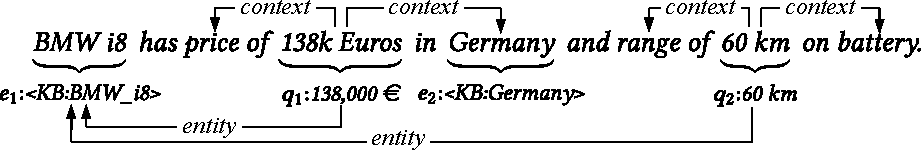
\includegraphics[width=0.5\textwidth]{figures/example_2}
\vspace{-2em}
\end{figure}

With the above example, we can extract two Qfacts: $\mathcal{F}_1 = (e = \textit{<KB:BMW\_i8>}; q = \textit{(138.000; \euro)}; X = \{\textit{price}, \textit{Germany}\})$ and $\mathcal{F}_2 = (e = \textit{<KB:BMW\_i8>}; q=\textit{(60; km)}; X = \{\textit{range}, \textit{battery}\})$.
We extract seed Qfacts from three large collections of text documents - the STICS project \cite{DBLP:conf/sigir/HoffartMW14}, the New York Times archive \cite{nyt}, and English Wikipedia, 
% \footnote{\url{https://meta.wikimedia.org/wiki/Data_dump_torrents\#English_Wikipedia}}
 containing a total of 13.4M documents. Extracted Qfacts from text are filtered by confidence, duplicate-removed, organized and indexed to serve the column alignment task 
 on web tables later.


\end{comment}